\documentclass[12pt]{article}
\usepackage{graphicx}
\usepackage[a4paper, margin=1.5cm]{geometry}
\usepackage[colorlinks=true, allcolors=blue]{hyperref}
\usepackage{url}
\usepackage{float}

\title{DT2470 Music Informatics Final Project}
\date{October 2025}

\author{
    \begin{minipage}[t]{0.24\textwidth}
        \centering
        Matei Cananau \\
        MSc in ML \\
        \href{mailto:cananau@kth.se}{cananau@kth.se}
    \end{minipage}
    \hfill
    \begin{minipage}[t]{0.24\textwidth}
        \centering
        Arvid Ljung \\
        MSc in ML \\
        \href{mailto:arvidlju@kth.se}{arvidlju@kth.se}
    \end{minipage}
    \hfill
    \begin{minipage}[t]{0.24\textwidth}
        \centering
        Matej Priesol \\
        MSc in ML \\
        \href{mailto:priesol@kth.se}{priesol@kth.se}
    \end{minipage}
    \hfill
    \begin{minipage}[t]{0.24\textwidth}
        \centering
        Bailin Lei \\
        MSc in ML \\
        \href{mailto:bailin@kth.se}{bailin@kth.se}
    \end{minipage}
}

\begin{document}

\maketitle

%% TABLE OF CONTENTS
\tableofcontents

\newpage

%% INTRODUCTION
\section{Introduction}

Earlier this year, Apple Music introduced their new "AutoMix" feature, which automatically creates smooth transition mixes between songs in a playlist. \cite{apple2025}. No public information is available regarding the technical details of this feature, except that it uses Apple Intelligence to apply time stretching and beat matching techniques.

A few months later, Spotify launched their own audio mixing function, allowing users to manually create DJ-style transitions between tracks in their playlists from one tempo and key pairing into another \cite{spotify2025}.

This project attempts to achieve similar functionality by extracting features from audio tracks and using MIR techniques to create smooth transitions between songs. The definition of a smooth transition was decided to mean one song that musically morphs into the next.

The full code can be accessed on Github, as a Python Notebook or in PDF format \cite{github_repo}. Resulting audio is found as the \textit{output.wav} file. Additionally, the group presentation is available in Google Slides \cite{presentation}.

%% FEATURE EXTRACTION
\section{Feature Extraction}

To create smooth transitions between the songs, we first needed to extract several features that would help us find the most natural points to start the transition, as well as determine how to best overlap the songs. For most of the features, the \textit{librosa} library was used.

The first thing we looked at was tempo and beat detection. This step determines the overall tempo (in beats per minute) and the exact time locations of beats. This was achieved by using an onset strength to estimate the global tempo and then picking the peaks that align with the estimated tempo. Both of these features were really accurate for all the songs. This was later used to time-stretch the song so that their beats and tempo align more naturally during the transition. Additionally, we also detect the downbeats. We assumed 4/4 time signature as all our songs followed it, and made a simplifying assumption that the starting beat is the downbeat.

Next, we tried to estimate the key of the song. This detection method analyzed the average chroma profile and compared the result with major and minor key templates, to determine the most likely one. However, key estimation is fairly difficult, so the key detection made some expected mistakes, like confusing B minor and D major as they are relative keys. But for the purpose of pitch matching, the performance was sufficient.

We also compute the Root Mean Square (RMS) energy of each song. This quantifies the amplitude of the signal over time, providing an estimate of its power/loudness. The song is divided into very short frames and the square root of the average squared amplitude for each frame is computed. This helped us to identify high and low energy regions in the song, so we can better determine the point where to start the transition, as it allows for smooth change between the energy levels of the two songs.

Finally, we performed structural segmentation to split the song into sections corresponding to intro, verse, chorus, and outro. This was achieved by computing a self-similarity matrix using the chroma features, in order to find sharp changes in the song, likely corresponding for the transition points between different song parts. 


\section{Transition scoring and generating outputs}

To find the optimal place to mix song A with song B, a set of candidate transitions is required. This involves the identification of multiple potential anchor points that could serve as the center of the crossfade. Each of these candidate points is then evaluated and assigned a similarity score to determine its quality. 

To calculate the score, we use dynamic time warping because it effectively measures how well the harmonic and rhythmic structures of Song A's outro align with those of Song B's intro. We also compare the musical keys of both songs, where transitions between compatible keys receive a higher score because they generate a more pleasing transition. The energy similarity is then measured using RMS loudness. Here, a smaller difference in energy between the end of Song A and the beginning of Song B is preferred, since this prevents a big jump or drop in volume during the mix. The candidate transitions that achieve the highest similarity score are then selected for use when generating the final smooth transition.

When generating the outputs, we begin by slicing the audio to define three main audio segments. In order to make a smooth transition, we must modify A's overlap to sound like B's overlap. We do this using strategies like tempo, pitch, and loudness matching. After that, an equal power crossfade is performed, where as song A fades out, song B fades in. It is used since it keeps the combined energy of the mix constant, which makes the transition feel smoother. The group found that the crossfade has the unwanted ability of overshadowing the other parts of the transition. As the focus lies in morphing one song into another, the crossfade had to be manually adjusted in a way that feels less intrusive.



%% EVALUATION
\section{Evaluation}

Evaluating transitions is a rather abstract task, as the point of transitions is to simply sound nice, not necessarily be mathematically correct. Musical smoothness depends on a balance of rhythm, loudness, and harmony, which is not always understood by numerical measures alone.

Despite this, some quantitative metrics such as beat phase error, tempo difference, loudness ratio and key distance were used to show an objective evaluation of the transition quality. These values indicate whether the characteristics of song A have been successfully adapted to morph into song B.

Nevertheless, subjective perception remained the most important criterion. Multiple combinations of songs and overlap durations were tested through listening, and the final pairing was chosen based on its perceptual smoothness and musicality. The results in the following section show both the quantitative findings and subjective perceptions of transition quality.

From the group's testing, a smooth transition was best achieved when song A was \textit{Billie Jean} by Michael Jackson and song B \textit{Get Lucky} by Daft Punk.



\section{Results}

\begin{figure}[H]
    \centering
    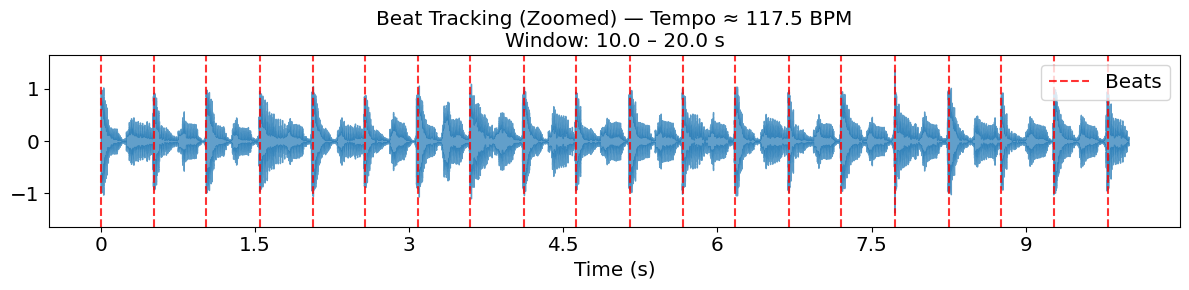
\includegraphics[width=\textwidth]{figures/beat_tracking_bj.png}
    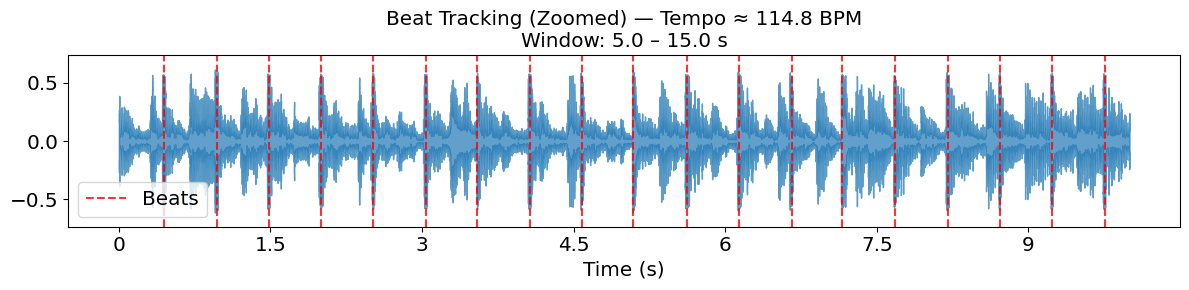
\includegraphics[width=\textwidth]{figures/beat_tracking_gl.png}
    \caption{Beat tracking for Billie Jean and Get Lucky.}
\end{figure}

\begin{figure}[H]
    \centering
    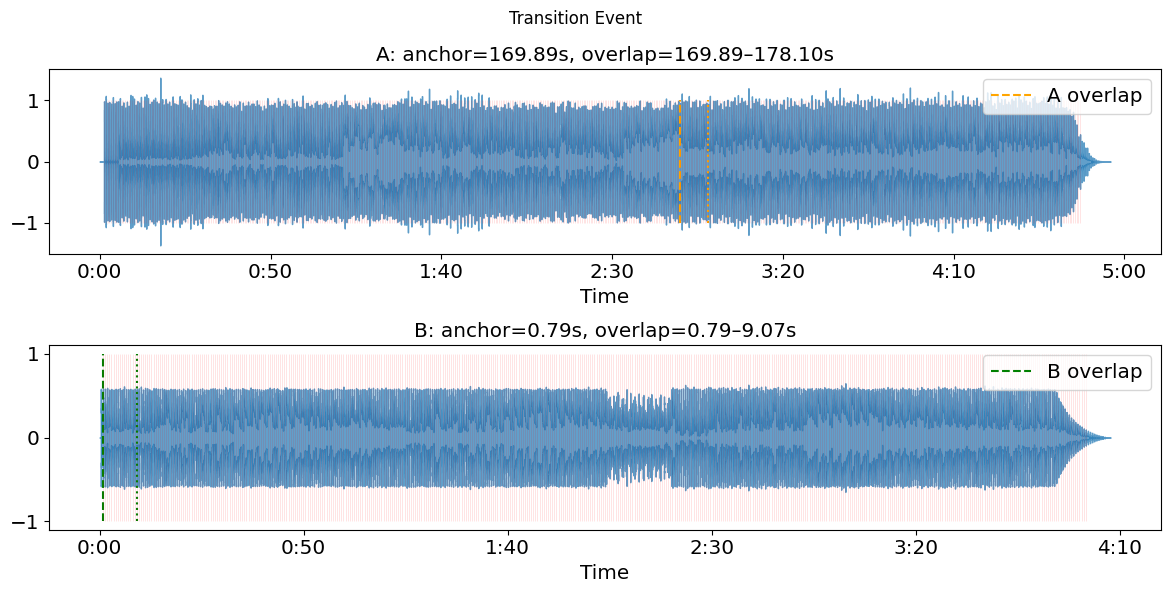
\includegraphics[width=\textwidth]{figures/transition.png}
    \caption{Transition anchor for songs A and B.}
\end{figure}

\begin{figure}[H]
    \centering
    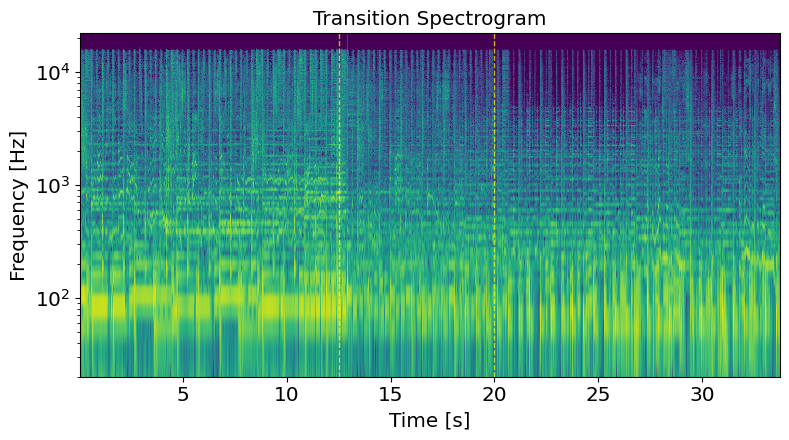
\includegraphics[width=\textwidth]{figures/spectogram.png}
    \caption{Transition spectrogram. Yellow lines show transition start and end.}
\end{figure}



\begin{table}[H]
\centering
\begin{tabular}{l l p{5.5cm}} 
\hline
\textbf{Metric} & \textbf{Value} & \textbf{Interpretation} \\
\hline
Anchor A (s) & 169.889 & Transition starts a little after the middle of song A. \\
Anchor B (s) & 0.789 & Transition begins just after the start of Song B. \\
Beat-phase error & 0.0 & Perfect beat alignment, continuous rhythm. \\
Tempo A (BPM) & 117.45 & Song A tempo. \\
Tempo B (BPM) & 114.84 & Song B tempo. \\
$\Delta$ Tempo (BPM) & 2.61 & Small tempo gap. \\
A tail RMS & 0.266 & Loudness at the end of Song A. \\
B head RMS & 0.137 & Loudness at the start of Song B. \\
Target overlap RMS range & [0.123, 0.279] & Overlap stays within intended loudness range. \\
Loudness diff (dB) & 5.78 & Slight mismatch but acceptable. \\
Key distance (semitones) & 5 & Moderate tonal change. \\
Same mode (maj/min) & True & Both songs share the same mode. \\
\hline
\textbf{Overall} & \textbf{Good transition quality} & Numerically and subjectively good transition. \\ 
\hline
\end{tabular}
\caption{Evaluation of the transition between Song A and Song B.}
\label{tab:evaluation}
\end{table}





\section{Areas of improvement}

Given the short amount of time given for this final project, many areas of improvement exist.

Firstly, testing out multiple songs gave rather different results. None were bad, but some better than others. The selected result of Billie Jean transitioning into Get Lucky gave the most satisfying result. Previously the song Under Pressure was meant to transition into Billie Jean. The group hypothesized that the finger snapping to the beat at the end of Under Pressure would produce a good transition into the solo drum and bass combo from the beginning of Billie Jean. However, as the BPM was close and the pitch was simple for  both the finger snapping and drum beat, the transition did not prove too much. Using more complex examples, such as the chosen two songs, gave a better understanding of the transition happening. Therefore, it is safe to assume that other songs would be even more interesting to build the transition between.

Secondly, the structure was only taken into account during the feature visualization section in order for the group to understand the look of each waveform. However, the structure was not used in the transition. Currently, the transition happens a little after the middle of song A, into the beginning of song B. In a real setting, e.g. when listening on a music platform, the transitions would strictly happen during the end of one song into the beginning of another. Our application did not necessarily focus on music platforms, however, but simply providing a generally good-sounding transition.

Thirdly, a subjective ranking was found to be of interest, a larger sample size would be beneficial.

Lastly, the transition was computed specifically to morph song A into song B. However, for a better effect, the transition would improve by the transition consisting of both a morphed song A and song B. This means that, currently, only song A is actually shifted to fit song B, with no shift happening to song B. A theory proposed by the group is developing a transition where the first half morphs A into B, while B is completely morphed into A. The latter half would continuously morph A into B, while B starts sounding more like the original. This would make the model more robust and hopefully fit a larger amount of different song choices.







%% REFERENCES
\bibliographystyle{plainurl}
\bibliography{references}

\end{document}